\documentclass[]{article}
\usepackage{amsmath, amsfonts, amssymb, amsthm}
\usepackage{cancel}
\usepackage{pgfplots}
\usepackage[output-complex-root=j]{siunitx}
\usepackage[american]{circuitikz}
\usepackage{bm}
\usepackage{graphicx}
\usepackage{fullpage}
\usepackage{pdfpages}

\renewcommand{\thesection}{\arabic{section}}
\renewcommand{\thesubsection}{\thesection.\alph{subsection}}
\renewcommand{\thesubsubsection}{\thesubsection.\roman{subsubsection}}
\renewcommand{\tilde}{\widetilde}

\newtheorem{genthm}{Theorem}

\title{EECS 16B HW04}
\author{Bryan Ngo}
\date{2020-02-25}

\begin{document}

\maketitle

\section{Phasors}

\subsection{}

\begin{align}
	Z_R &= R = \SI{1.5}{\ohm} \\
	Z_C &= \frac{1}{j \omega C} = -\frac{j}{\omega} \, \si{\ohm} \\
	Z_L &= j \omega L = j \omega \, \si{\ohm}
\end{align}

\subsection{}

\begin{center}
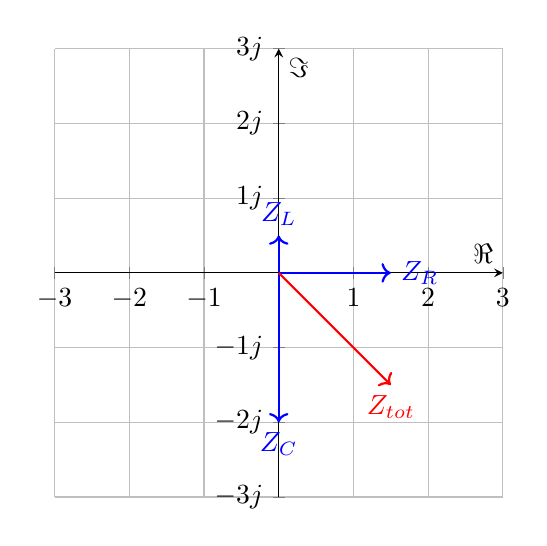
\begin{tikzpicture}
	\begin{axis}[
		xlabel = {\(\Re\)},
		ylabel = {\(\Im\)},
		xmin = -3, xmax = 3,
		ymin = -3, ymax = 3,
		xtick = {-3,...,3},	ytick = {-3,..., 3},
		yticklabel = {\(\pgfmathprintnumber{\tick}j\)},
		axis lines = middle,
		grid = major,
		axis equal image
	]
		\addplot[thick, color=blue, ->] coordinates{
			(0, 0) (1.5, 0)
		} node[right]{\(Z_R\)};
		\addplot[thick, color=blue, ->] coordinates{
			(0, 0) (0, -2)
		} node[below]{\(Z_C\)};
		\addplot[thick, color=blue, ->] coordinates{
			(0, 0) (0, 0.5)
		} node[above]{\(Z_L\)};
		\addplot[thick, color=red, ->] coordinates{
			(0, 0) (1.5, -1.5)
		} node[below]{\(Z_{tot}\)};
	\end{axis}
\end{tikzpicture}
\end{center}

\begin{gather}
	|Z_{tot}| = 1.5 \sqrt{2} \, \si{\ohm} \\
	\theta = -\frac{\pi}{4} \, \si{\radian}
\end{gather}

\subsection{}

\begin{center}
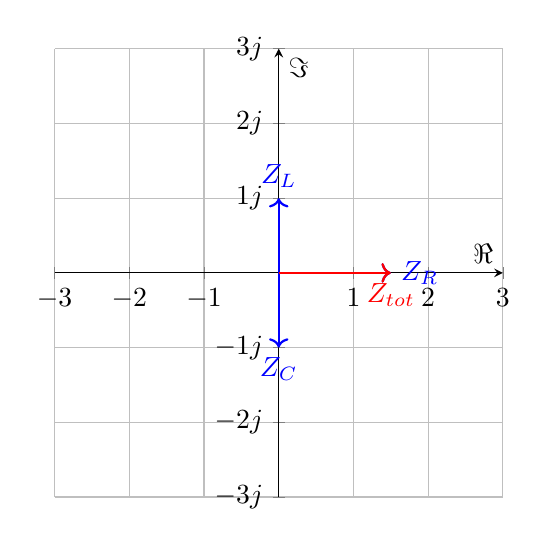
\begin{tikzpicture}
	\begin{axis}[
		xlabel = {\(\Re\)},
		ylabel = {\(\Im\)},
		xmin = -3, xmax = 3,
		ymin = -3, ymax = 3,
		xtick = {-3,...,3},	ytick = {-3,..., 3},
		yticklabel = {\(\pgfmathprintnumber{\tick}j\)},
		axis lines = middle,
		grid = major,
		axis equal image
	]
		\addplot[thick, color=blue, ->] coordinates{
			(0, 0) (1.5, 0)
		} node[right]{\(Z_R\)};
		\addplot[thick, color=blue, ->] coordinates{
			(0, 0) (0, -1)
		} node[below]{\(Z_C\)};
		\addplot[thick, color=blue, ->] coordinates{
			(0, 0) (0, 1)
		} node[above]{\(Z_L\)};
		\addplot[thick, color=red, ->] coordinates{
			(0, 0) (1.5, 0)
		} node[below]{\(Z_{tot}\)};
	\end{axis}
\end{tikzpicture}
\end{center}

\begin{gather}
	|Z_{tot}| = \SI{1.5}{\ohm} \\
	\theta = \SI{0}{\radian}
\end{gather}

\subsection{}

\begin{center}
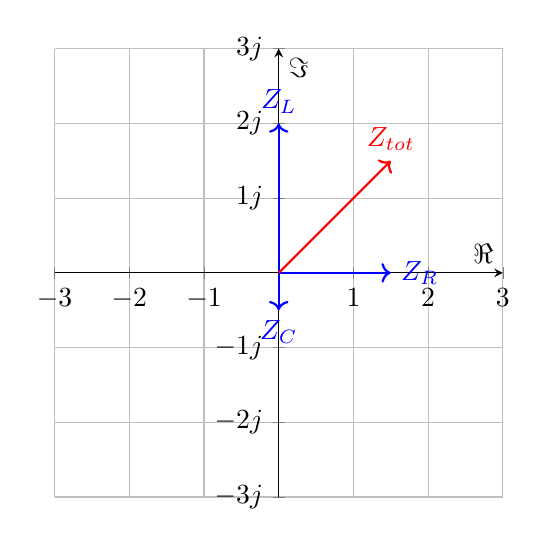
\begin{tikzpicture}
	\begin{axis}[
		xlabel = {\(\Re\)},
		ylabel = {\(\Im\)},
		xmin = -3, xmax = 3,
		ymin = -3, ymax = 3,
		xtick = {-3,...,3},	ytick = {-3,..., 3},
		yticklabel = {\(\pgfmathprintnumber{\tick}j\)},
		axis lines = middle,
		grid = major,
		axis equal image
	]
		\addplot[thick, color=blue, ->] coordinates{
			(0, 0) (1.5, 0)
		} node[right]{\(Z_R\)};
		\addplot[thick, color=blue, ->] coordinates{
			(0, 0) (0, -0.5)
		} node[below]{\(Z_C\)};
		\addplot[thick, color=blue, ->] coordinates{
			(0, 0) (0, 2)
		} node[above]{\(Z_L\)};
		\addplot[thick, color=red, ->] coordinates{
			(0, 0) (1.5, 1.5)
		} node[above]{\(Z_{tot}\)};
\end{axis}
\end{tikzpicture}
\end{center}

\begin{gather}
	|Z_{tot}| = 1.5 \sqrt{2} \, \si{\ohm} \\
	\theta = -\frac{\pi}{4} \, \si{\radian}
\end{gather}

\subsection{}

\(\omega_n = \SI{1}{\radian\per\second}\)

\section{Low-pass Filter}

\begin{center}
\begin{circuitikz}\draw
	(0, 2) to[sV_=\(V_{in}\)] (0, 0)
	(0, 2) to[R=\SI{1}{\kilo\ohm}] (2, 2) to[C=\SI{1}{\micro\farad}] (2, 0) node[ground]{} to[short] (0, 0)
	(2, 2) to[short] (4, 2) to[open, v^=\(V_{out}\), o-o] (4, 0) to[short] (2, 0)
;\end{circuitikz}
\end{center}

\subsection{}

Phasorizing, the circuit is now transformed into

\begin{center}
\begin{circuitikz}\draw
	(0, 2) to[sV_=\(\tilde{V}_{in}\)] (0, 0)
	(0, 2) to[R=\SI{1}{\kilo\ohm}] (2, 2) to[C=\(\frac{1}{j \omega (\SI{1}{\micro\farad})} \, \si{\ohm}\)] (2, 0) node[ground]{} to[short] (0, 0)
	(2, 2) to[short] (4, 2) to[open, v^=\(\tilde{V}_{out}\), o-o] (4, 0) to[short] (2, 0)
;\end{circuitikz}
\end{center}

\subsection{}

\begin{equation}
	H(j \omega) = \frac{\tilde{V}_{out}}{\tilde{V}_{in}} = \underbrace{\frac{\frac{1}{j \omega (\SI{1}{\micro\farad})}}{\SI{1}{\kilo\ohm} + \frac{1}{j \omega (\SI{1}{\micro\farad})}}}_{\text{voltage divider}} = \frac{1}{1 + (\SI{1}{\kilo\ohm}) j \omega (\SI{1}{\micro\farad})} = \frac{1}{1 + j \omega (\SI{1}{\milli\second})}
\end{equation}

\subsection{}

\begin{gather}
	H(\SI{jd+6}{\radian\per\second}) = \frac{1}{1 + (\SI{jd+6}{\radian\per\second}) (\SI{1}{\milli\second})} = \frac{1}{1 + \num{jd+3}} \approx \num{0.001+jd-3} \\
	\Rightarrow |H(\SI{jd+6}{\radian\per\second})| \approx \SI{d-3}{\ohm}
\end{gather}

\subsection{}

\begin{gather}
	H(\SI{j}{\radian\per\second}) = \frac{1}{1 + (\SI{j}{\radian\per\second}) (\SI{1}{\milli\second})} = \frac{1}{1 + \num{jd-3}} \approx \num{1+0.001jd-3} \\
	\angle H(\SI{j}{\radian\per\second}) \approx \SI{-d-3}{\radian}
\end{gather}

\subsection{}

Since the input is a sine wave, our input \(V_{in}(t) = \Re\{e^{j \frac{\pi}{2}} e^{1000jt}\}\).
Then,
\begin{align}
	\left.\tilde{V}_{out}\right|_{\omega = 1000} &= \frac{1}{1 + j} \tilde{V}_{in} \\
	V_{out}(t) &= \Re\left\{\tilde{V}_{out} e^{1000jt}\right\} \\
	&= \Re\left\{\frac{1}{1 + j} \tilde{V}_{in} e^{1000jt}\right\} \\
	&= \Re\left\{\frac{1}{1 + j} e^{j \frac{\pi}{2}} e^{1000jt}\right\} \\
	&= \Re\left\{\frac{1}{|1 + j|} e^{-j \frac{\pi}{4}} e^{j \frac{\pi}{2}} e^{1000jt}\right\} \\
	&= \frac{1}{\sqrt{2}} \cos\left(1000t + \frac{\pi}{4}\right)
\end{align}

\subsection{}

\begin{center}
	\begin{minipage}{0.5\textwidth}
		\includegraphics[width=\linewidth]{bode_mag}
	\end{minipage}\hfill
	\begin{minipage}{0.5\textwidth}
		\includegraphics[width=\linewidth]{bode_phase}
	\end{minipage}
\end{center}

\section{Color Organ Filter Design}

\subsection{}

For the low-pass filter, the cutoff frequency is
\begin{equation}
	f_{cut} = \frac{1}{2 \pi RC} \Rightarrow R = \frac{1}{2 \pi f_{cut} C} = \SI{66}{\ohm}
\end{equation}
For the high-pass filter,
\begin{equation}
	f_{cut} = \frac{1}{2 \pi RC} \Rightarrow R = \frac{1}{2 \pi f_{cut} C} = \SI{1.6}{\kilo\ohm}
\end{equation}

\begin{center}
\begin{circuitikz}\draw
	(0, 2) to[sV_=\(V_{in}\)] (0, 0)
	(0, 2) to[R=\SI{66}{\ohm}] (2, 2) to[C=\SI{1}{\micro\farad}] (2, 0) to[short] (0, 0)
	(2, 2) to[short] (4, 2) to[open, v^=\(V_{out1}\), *-*] (4, 0) node[ground]{} to[short] (2, 0)
	(4, 2) to[C=\SI{1}{\micro\farad}] (6, 2) to[R=\SI{1.6}{\kilo\ohm}] (6, 0) to[short] (0, 0)
	(6, 2) to[short] (8, 2) to[open, v^=\(V_{out2}\), o-o] (8, 0) to[short] (6, 0)
;\end{circuitikz}
\end{center}

\subsection{}

Since there is no buffer, we cannot simply take the product.
Using equivalent impedance, the voltage \(V_{out1}\) is
\begin{equation}
	V_{out1} = \frac{(R_H + \frac{1}{j \omega C_H}) \parallel \frac{1}{j \omega C_L}}{(R_H + \frac{1}{j \omega C_H}) \parallel \frac{1}{j \omega C_L} + R_L} V_{in}
\end{equation}
Meaning that
\begin{equation}
	V_{out2} = \frac{j \omega R_H C_H}{1 + j \omega R_H C_H} \frac{(R_H + \frac{1}{j \omega C_H}) \parallel \frac{1}{j \omega C_L}}{(R_H + \frac{1}{j \omega C_H}) \parallel \frac{1}{j \omega C_L} + R_L} V_{in}
\end{equation}

\subsection{}

\begin{center}
	\begin{minipage}{0.5\textwidth}
		\includegraphics[width=\linewidth]{3c_mag}
	\end{minipage}\hfill
	\begin{minipage}{0.5\textwidth}
		\includegraphics[width=\linewidth]{3c_phase}
	\end{minipage}
\end{center}
The numerator becomes zero when \(\omega = 0\).
The denominator becomes 0 when \(\omega = \frac{j}{R_L C_L}, \frac{j}{R_H C_H}\).
The maximum magnitude is 0, which makes sense because we cannot amplify the signal with passive elements.

\subsection{}

First, we find \(K_{mic}\), which is
\begin{align}
	\frac{1}{2} V_{pp} &= K_{mic} \frac{j \omega \left(1 + \frac{j \omega}{\omega_{z1}}\right)}{\left(1 + \frac{j \omega}{\omega_{p1}}\right) \left(1 + \frac{j \omega}{\omega_{p2}}\right) \left(1 + \frac{j \omega}{\omega_{p3}}\right)} \\
	\Rightarrow K_{mic} &= \frac{\left(1 + \frac{j \omega}{\omega_{p1}}\right) \left(1 + \frac{j \omega}{\omega_{p2}}\right) \left(1 + \frac{j \omega}{\omega_{p3}}\right)}{2j \omega \left(1 + \frac{j \omega}{\omega_{z1}}\right)} V_{pp} \approx \SI{8.6-0.5j}{\milli\volt}
\end{align}
Then, we plug \(V_{mic}\) as the input voltage into the filters,
\begin{align}
	V_{LP} &= \frac{2}{1 + \frac{j \omega}{200 \pi}} V_{mic} \\
	V_{BP} &= \frac{\num{4.54d-4} j \omega}{\left(1 + \frac{j \omega}{400 \pi}\right) \left(1 + \frac{j \omega}{4000 \pi}\right)} V_{mic} \\
	V_{HP} &= \frac{\frac{j \omega}{8000 \pi}}{1 + \frac{j \omega}{8000 \pi}} V_{mic}
\end{align}

\subsection{}

With \(V_{pp} = \SI{5}{\volt}\), we want our amplitude of the phasor to be \SI{2.5}{\volt} outside the amplifier.
Thus, \(G = \frac{2.5}{|V_{out}|}\).
At \SI{50}{\hertz},
\begin{align}
	|V_{LP}(2 \pi \cdot 50)| \approx \SI{1.76}{\volt} \Rightarrow G &= 1.42 \\
	|V_{BP}(2 \pi \cdot 50)| \approx \SI{0.136}{\volt} \Rightarrow G &= 18.4 \\
	|V_{HP}(2 \pi \cdot 50)| \approx \SI{12.3}{\milli\volt} \Rightarrow G &= 203
\end{align}
At \SI{1000}{\hertz},
\begin{align}
	|V_{LP}(2 \pi \cdot 1000)| \approx \SI{0.109}{\volt} \Rightarrow G &= 22.9 \\
	|V_{BP}(2 \pi \cdot 1000)| \approx \SI{0.275}{\volt} \Rightarrow G &= 9.09 \\
	|V_{HP}(2 \pi \cdot 1000)| \approx \SI{0.133}{\volt} \Rightarrow G &= 18.7
\end{align}
At \SI{8000}{\hertz},
\begin{align}
	|V_{LP}(2 \pi \cdot 8000)| \approx \SI{10.6}{\milli\volt} \Rightarrow G &= 235 \\
	|V_{BP}(2 \pi \cdot 8000)| \approx \SI{58.8}{\milli\volt} \Rightarrow G &= 42.5 \\
	|V_{HP}(2 \pi \cdot 1000)| \approx \SI{0.380}{\volt} \Rightarrow G &= 6.57
\end{align}

\section{Mystery Microphone}

\subsection{}

The microphone is most sensitive at frequencies \SI{3d+2}{\hertz}---\SI{5d+3}{\hertz}.
The microphone is least sensitive mostly everywhere else, particularly \SI{10}{\hertz}---\SI{70}{\hertz}.

\subsection{}

You would have the best time hearing the mid-range frequencies, since the mic is most responsive to those frequencies, and have a harder time hearing the lower-end and higher-end frequencies.

\subsection{}

I would apply an amplification block for frequencies \SI{10}{\hertz}---\SI{70}{\hertz} with an amplifier gain of \(12.5\).
I would also apply an amplification block for frequencies above \SI{d+4}{\hertz} with an amplifier gain of \(1.67\).

\stepcounter{section}

\section{Homework Process and Study Group}

\begin{enumerate}
	\item I used lecture note 2020-02-13 and Note 5.
	\item I worked on this homework by myself.
	\item I worked on this homework in one sitting.
	\item 4 hours.
\end{enumerate}

\newpage

%\includepdf[pages=-]{prob*.pdf}

\end{document}
